\documentclass[10pt]{article}

\usepackage{parskip}
\usepackage[margin=1in]{geometry} 
\usepackage{tikz}
\usetikzlibrary{positioning}
\usepackage{amsmath,amsthm,amssymb, graphicx, multicol, array}
\usepackage{enumitem}
\usepackage{amssymb}
\usepackage{float}
\usepackage{href-ul}
 
\newcommand{\N}{\mathbb{N}}
\newcommand{\Z}{\mathbb{Z}}
 
\newenvironment{problem}[2][Problem]{\begin{trivlist}
\item[\hskip \labelsep {\bfseries #1}\hskip \labelsep {\bfseries #2.}]}{\end{trivlist}}

\begin{document}
 
\title{Difference-in-difference}
\author{Jakob Sverre Alexandersen\\
GRA4158 Marketing and the Analysis of Experiments and Quasi-Experiments\\
Lecture 11}
\maketitle

\tableofcontents
\newpage
\section{Overview}
\begin{itemize}
    \item Treatment cannot be randomized 
    \item Time-series available:
    \item DID 
    \item Synthetic control + advancements 
    \item Regression discontinuity design (RDD)
\end{itemize}
\textbf{Non-random assignment}
\begin{itemize}
    \item We are still in quasi-experimental or observational settings 
    \begin{itemize}
        \item We have non-rando assignment $\to $ there are selection effects 
    \end{itemize}
    \item we still want to estimate causal effects 
    \item The problem with regression, matching, weighting, DML etc: 
    \begin{itemize}
        \item They all require conditional independence (unconfoundedness)
        \item They require that ALL necessary covariates to capture the selection mechanism are known and measured 
        \item No selection on observables 
        \item Unrealistic in many situations 
    \end{itemize}
\end{itemize}
\section{The aspect of time}
\begin{itemize}
    \item So far, we have been mostly looking at outcomes after treatment 
    \begin{itemize}
        \item Treated group realizes potential outcomes $Y_i(1) $
        \item Untreated group realizes potential outcomes $Y_i(0) $ with $i \neq j $
    \end{itemize}
    \item Cross-sectional data 
    \begin{itemize}
        \item Observations are collected from many different subjects at a single point in time -- here after treatment
    \end{itemize}
    \item Time-series data / panel data / multi-level data 
    \begin{itemize}
        \item Multiple observations for an individual 
        \begin{itemize}
            \item e.g., single unit across multiple points in time 
            \item e.g., different units at multiple points in time 
            \item e.g., nested multi-level data (e.g., students nested within schools, firms nested within countries)
        \end{itemize}
    \end{itemize}
    \item Example: weekly sales at different stores
\end{itemize}
\begin{center}
    \begin{tabular}{|c|c|c|c|c|}
        \hline 
        & Week 1 & Week 2 & $\dots$ & Week $t$\\\hline 
        Store 1 & $x_{11}$ & $x_{12} $ & $\dots$ & $x_{1t} $\\\hline 
        Store 2 & $x_{21}$ & $x_{22} $ & $\dots$ & $x_{2t} $\\\hline 
        $\vdots $ &$\vdots $ &$\vdots $ &$\ddots $ &$\vdots $ \\\hline
        Store s & $x_{s1}$ & $x_{s2} $ & $\dots$ & $x_{st} $\\\hline 
    \end{tabular}
\end{center}
\newpage 
\section{Recap: panel data -- fixed effect model}
\begin{itemize}
    \item $Y_{st} = \mu_s + \tau_t + \beta_1T_{st} + \epsilon_{st} $
    \begin{itemize}
        \item $\mu_s $ is the store-level fixed effect 
        \begin{itemize}
            \item All unobserved characteristics of the cross-sectional unit (the store) that vary over $ s $ but not over $t $
            \item Differences between stores that are stable over time 
        \end{itemize}
        \item $\tau_t $ is the time-period fixed effect 
        \begin{itemize}
            \item Unobserved time varying effects; varies across time $t $ but not across $s $ (stores)
            \item Differences over time that are stable across stores 
        \end{itemize}
    \end{itemize}
    \item It is relatively easy to estimate / eliminate $\mu_s \text{ and } \tau_t $ if we have sufficient data on both the time and subject dimension (e.g., dummy variables, demeaning, first-differences, etc.)
    \item $\beta_1 $ is consistent if $\text{cov}(T_{st}, \epsilon_{st} = 0 ) $ after controlling for $\mu_s \text{ and } \tau_t $.
    \item Panel data solves the endogeneity problem that arises from time-invariant or subject-invariant unobserved effects 
    \item Typical subject-specific components 
    \begin{itemize}
        \item Quality of products, location of stores, management capabilities of firms, culture within firms 
        \item Characteristics of regions, countries, \dots 
        \item Individual customer characteristics 
        \item Subject fixed-effects are sufficient as long as these characteristics do not vary over time (within the time-frame under investigation)
    \end{itemize}
    \item Typical time-varying components
    \begin{itemize}
        \item Seasonality, trend, holidays 
        \item Events (political, spots), changes in legislation 
        \item Time fixed-events are sufficient as long as these events affect all cross-sectional units (e.g., all stores) the same way 
    \end{itemize}
\end{itemize}
\section{Recap: panel data -- remaining endogeneity problems}
\begin{itemize}
    \item Oanel data (or multi-level data more generally) is already a very powerful way of addressing a wide range of endogeneity concerns 
    \item Problems that remain: time and subject specific omitted variables and reverse causality
    \begin{itemize}
        \item Unobserved characteristics of the cross-section units $s $ that vary over time $ t $ and correlate with $T_s \to $ i.e., $X_{st} $ with $\text{cov}(X_{st}, T_{st}) \neq 0 $ and influence $Y_{st} $
        \item The outcome variable in a period (or more typically the expectation of it) influences the treatment assignment $T_{st} $
        \begin{itemize}
            \item e.g., local and time dependent events that influence sales and also influence treatment selection as managers expect higher/lower sales 
            \item e.g., loacl competitor behavior that is store specific and time varying and influences treatment selection
            \item e.g., treatment selection based on local trends (increasing or decreasing sales)
        \end{itemize}
    \end{itemize}
\end{itemize}
\newpage 
\section{Solutions (so far)}
\begin{itemize}
    \item If we are able to observe these variables, we should add them as controls 
    \begin{itemize}
        \item Selection on observables
        \item $Y_{st} = \mu_s + \tau_t + \beta_1 + T_{st} + \gamma X_{st} \epsilon_{st} $
        \item We can use regression analysis (typical panel estimators) or matching, weighting, DML 
    \end{itemize}
    \item If we are not able to observe these variables, we may use instrumental variables 
    \begin{itemize}
        \item Selection on unobservables 
        \item Instrumental variables would also need to vary over $s \text{ and } t $
        \item We can use 2SLS or the control function approach 
    \end{itemize}
\end{itemize}
\section{Difference-in-difference (DiD) framework}
\begin{itemize}
    \item We now focus on two groups with measurements before and after treatment 
    \begin{itemize}
        \item One group is treated, and the other is not (binary treatment)
    \end{itemize}
    \item Remember, within-subject framework utilizes potential outcomes before and after treatment for the same individual $i $ to calculate treatment effects 
    \begin{itemize}
        \item $\mathbb{E}[Y_{i, \text{post}}] - \mathbb{E}[Y_{i, \text{pre}}]$
        \item However, this difference only represents a causal effect if $Y_{i, \text{pre}}(0) = Y_{i, \text{post}}(0) $
        \begin{itemize}
            \item i.e., the counterfactual outcome does not change over time 
        \end{itemize}
        \item Typically, we cannot rule out that other factors contributed to pre - post difference
        \begin{itemize}
            \item Trends, events, policy changes etc. 
        \end{itemize}
    \end{itemize}
    \item We will now extend this idea, relaxing the assumption of no change over time to a more general parallel trends assumption 
\end{itemize}
\newpage
\section{DiD rationale}
\begin{itemize}
    \item Untangle the impact of the treatment from a general trend 
    \item What is the difference in outcomes that we would observe for the treated group (red line) relative to the counterfactual (black dotted line) if the trend that we observed for the control and treated group would continue?
    \item \textbf{Core idea:}
    \begin{itemize}
        \item There can be level differences between treatment and control (e.g., $\alpha_{g = 1} - \alpha_{g = 0} $), but the treatment units would have followed the same path parallel to the control units in the absence of treatment (e.g., $\delta_{\text{post}} - \delta_{\text{pre}} $)
        \item Common trend or parallel trend assumption 
    \end{itemize}
\end{itemize}
\begin{figure}[H]
    \centering
    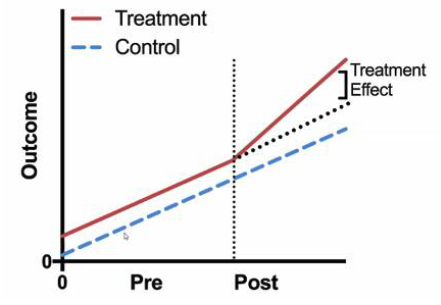
\includegraphics[width=0.5\textwidth]{2026-03-25-16-58-04.png}
\end{figure}
\section{Core of DiD framwork}
\begin{itemize}
    \item We assume additive structure for mean potential outcomes in case of no treatment: 
    \begin{gather*}
        \mathbb{E}[Y_{igt}(0)] = \delta_t + \alpha_g
    \end{gather*}
    \begin{itemize}
        \item There are effects of time $\delta_t $ and treatment group $\alpha_g $ and these are linearly separable 
    \end{itemize}
    \item Remember: we can represent the observed outcomes as a dunction of the potential outcomes: 
    \begin{gather*}
        Y_{igt} = Y_{igt}(1)T_{gt} + Y_{igt}(0) (1 - T_{gt})
    \end{gather*}
    \item Taking expectation and rewriting gives: 
    \begin{gather*}
        \mathbb{E}[Y_{igt}] = \beta T_{gt} + \delta_t + \alpha_g 
    \end{gather*}
    \item We compare outcomes for treated and control \textit{after} intervention 
    \item And compare outcomes for treated before and after intervention
    \item DiD estimator: 
    \begin{gather*}
        \text{ATET}_{\text{DID}} = \beta 
    \end{gather*}
\end{itemize}
\newpage 
\section{Common or parallel trend assumption}
\begin{itemize}
    \item For the simple 2 groups - 2 time points setting the assumption is formally given by
    \begin{gather*}
        \mathbb{E}[Y_{igt}(0)|t = \text{post}, g = 0] - \mathbb{E}[Y_{igt}(0)|t = \text{pre}, g = 0]
    \end{gather*}
    \begin{itemize}
        \item The difference between pre and post (potential) outcomes is equal between treatment and control group (and under the typical assumption of SUTVA this relates to observed outcomes)
    \end{itemize}
    \item What happens when the assumption fails?
    \begin{gather*}
        \text{ATET}_{\text{DID}} = \beta + (\text{difference in trends})
    \end{gather*}
\end{itemize}
More generally, 
\begin{itemize}
    \item while traditional independence assumption $\{Y_i(1), Y_i(0)\}\bot T_i $ states that the treatment assignment can't be related to the levels of potential outcomes 
    \begin{itemize}
        \item i.e., $\alpha_{g = 1} - \alpha_{g = 0} = 0 $ because this is $\mathbb{E}[Y_{it}(0)|g = 1] - \mathbb{E}[Y_{it}(0)|g = 0] = 0 $
        \item i.e., $\delta_{\text{post}} - \delta_{\text{pre}} = 0 $ because this is $\mathbb{E}[Y_{it}(0)|\text{post}] - \mathbb{E}[Y_{it}(0)|\text{pre}] = 0 $
    \end{itemize}
    \item The DiD relaxes this assumption and only requires that the treatment assignmetn can't be related to the growth in potential outcomes over time 
    \begin{gather*}
        \{Y_{i, t}(0) - Y_{i, t -1 }(0)\}\bot T_i \\
        \{\delta_t - \delta_{t - 1}\}\bot T_i
    \end{gather*}
\end{itemize}
\textbf{Example}
\begin{itemize}
    \item Simple setting: 2 groups - 2 time points
\end{itemize}
\begin{figure}[H]
    \centering
    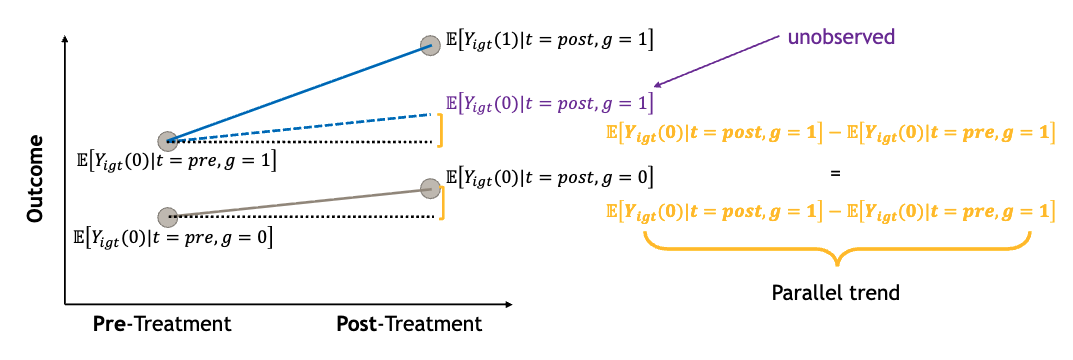
\includegraphics[width=0.8\textwidth]{2026-03-25-17-12-19.png}
\end{figure}
\begin{figure}[H]
    \centering
    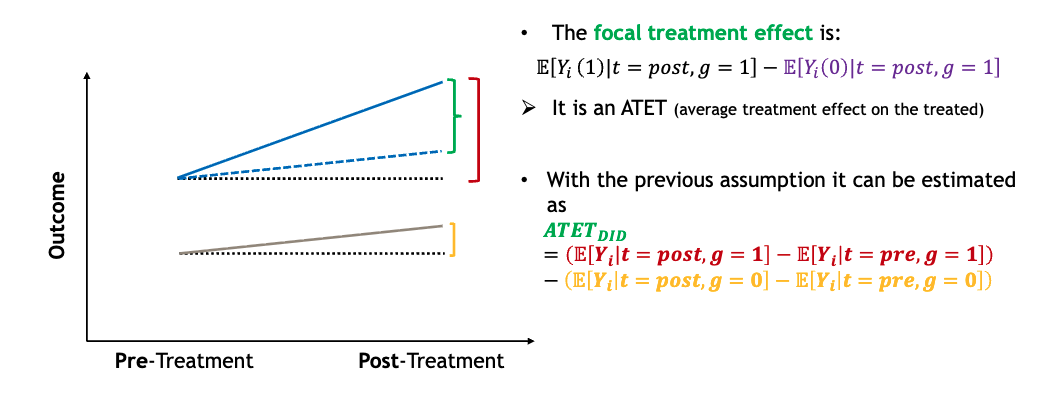
\includegraphics[width=0.8\textwidth]{2026-03-25-17-12-40.png}
\end{figure}
\newpage 
\section{Common trend assumption}
\begin{itemize}
    \item How to assess common trends?
    \begin{itemize}
        \item Graphical inspection of parallel trends in pre-treatment periods (figures like before)
        \item Estimating trend models on the pre-treatment periods and assessing the time trend differences between the control and treatment groups (e.g., using an interaction)
        \begin{itemize}
            \item $Y_{it} = \alpha + \gamma_1t + \gamma_2T_it + \xi_{it}\quad \text{for }t < \text{POST}_t $
        \end{itemize}
        \item Some studies use DiD in combination with some form of matching 
        \begin{itemize}
            \item e.g., create groups with matching trends 
        \end{itemize}
    \end{itemize}
\end{itemize}
\end{document}